%!TeX root = ../complex_net_report_senacheribbe.tex

\graphicspath{{../assignment4/figures/}}

\subsection{Introduction}
In this last assignment, we are required to implement the Barabási–Albert model and to test its properties. BA is a generative model, which means that the graph is defined through a process/algorithm and cannot be defined mathematically by associating a probability space (which can be done for instance for G(n,p)).
Simulations are therefore even more essential to study the properties of the model.

The main concept behind this model is the preferential attachment rule, according to which a new node that joins the network will be connected with higher probability to most popular nodes.
Indeed, we start from an initial graph and we add iteratively one node at a time and connect it to $m_{BA}$ nodes already in the graph (we didn't use the notation $m$ to avoid confusions with the number of edges). The probability $p_u$ for a new coming node to connect to a node $u$ in the graph is given by \cref{eq:pu_BA}
\begin{equation}
p_u = \frac{d_u^\gamma}{\sum_{v \in V}{d_v^\gamma}}\label{eq:pu_BA}
\end{equation}
where $d_u$ is the current degree of the node $u$ and $\gamma$ is the exponent that defines the proportion between $p_u$ and $d_u$.

\subsection{Algorithms}
We now present two different algorithms to create a BA graph. The first approach adopted, which is presented in \cref{algo:ba_opt}, is able to generate very efficiently a BA graph for the case $p_u \propto d_u$. It's employing essentially an additional vector ($urn$) which is constructed so that the number of times each node $i$ of the graph appears in the vector is equal to the $deg(i)$. Picking a random element from $urn$ corresponds then to sampling the discrete distribution described in \cref{eq:pu_BA} with $\gamma=1$.

The second approach (\cref{algo:ba}) instead computes the distribution each time and samples it, instead of employing an auxiliary vector. This method is more computationally expensive, but it's the only viable for the case $p_u \not\propto d_u$. To further optimize it, the cumulative distribution to perform the sampling from is not computed entirely, but just for the portion needed. Notice indeed in the function \textit{random\_choice} described in \cref{algo:ba_r_c} the use of $sum\_p_u=\sum_{u} p_u$, so that we don't have to loop over all nodes in $p_u$ to compute the sum and the \textit{while} in line 14 that stops as soon as a new value is picked.\\
With this optimisation, especially for the case $p_u \propto d_u^{\gamma}$ with $\gamma>1$, the sampling can be computed very fast, because the initial nodes are big hubs, usually chosen for the new edges. The computation of the distribution is therefore stopped after few iterations.
We reduced in this way the average case complexity, while the worst case one remains still the same.
 
\subsection{Results}
In \cref{fig:sparsity4}, we report the sparsity of the adjacency matrix of a Barabási–Albert graph generated with $n=1000$ and $m_{BA}=3$. As expected, older nodes (first rows and columns) have more connections (more dense points), since they had more chances to be chosen from new nodes.

\begin{figure} [!ht]
	\centering
	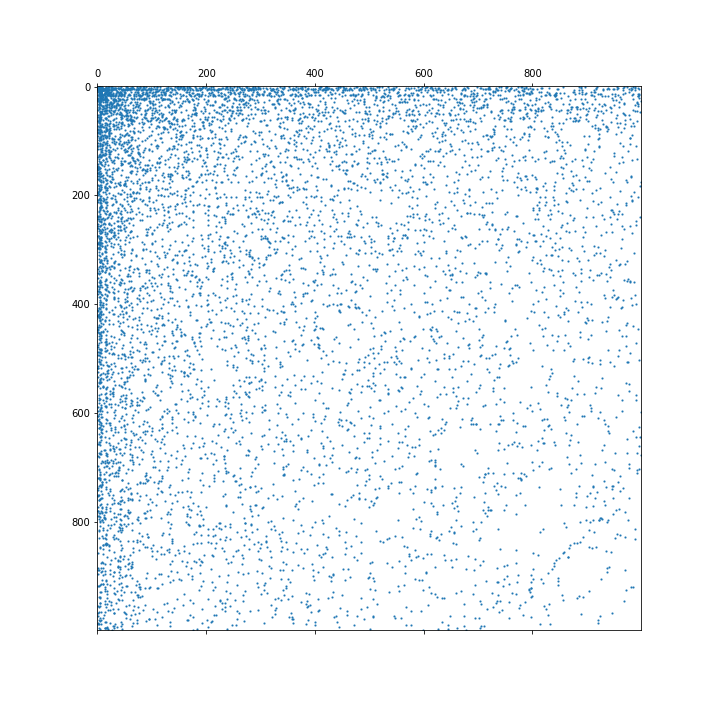
\includegraphics[width=.6\linewidth, clip, trim={2cm 2cm 2cm 2cm}]{sparsity}
	\caption{Sparsity of Barabási–Albert graph with $n=1000$, $m_{BA}=3$ and $m=3990$ (number of edges)}
	\label{fig:sparsity4}
\end{figure}
\pagebreak
The model was then run with $n=100000$ and $m_{BA}=3$, for the case $p_u \propto d_u$, $p_u \propto \sqrt{d_u}$ and $p_u \propto d_u^{1.5}$ (\cref{algo:ba_opt} was used for the case  $p_u \propto d_u$, while \cref{algo:ba} for the other two). For each of these functions of the degree, 100 graphs were generated. Following a Monte Carlo approach, the results shown in \cref{t:res4} and \cref{fig:deg4_gamma1,fig:deg4_gammacomp} are an average on those realisations.\\

\begin{table}[ht!]
	\centering
	\begin{tabular}{ |c|c|c|c| } 
		\hline
		gamma $\gamma$ & diameter &  clustering & max degree\\
		\hline
		1 & 7.54 & 0.000886 & 1540\\
		0.5 & 8.52 & 0.000120 & 110\\
		1.5 & 3.50 & 0.845655 & 97321\\
		\hline
	\end{tabular}
	\caption{Results for BA, $n=100000$,  $m_{BA}=3$, average from $100$ graphs for each $\gamma$}
	\label{t:res4}
\end{table}
\begin{figure} [!ht]
	\centering
	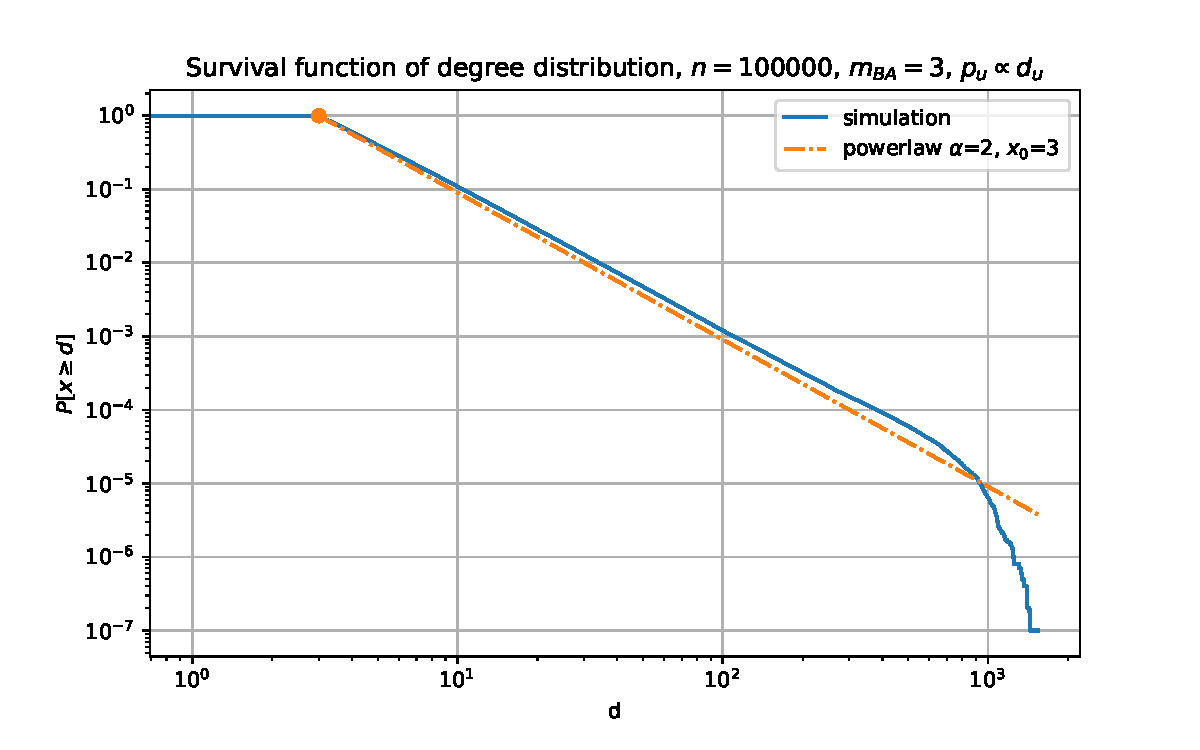
\includegraphics[width=.5\linewidth]{deg_gamma1}
	\caption{Survival function of degree distribution, BA with $n=100000$,  $m_{BA}=3$, $\gamma=1$}
	\label{fig:deg4_gamma1}
\end{figure}

The clustering coefficient is computed approximately by taking at random 50000 nodes, and for each node picking 2 random neighbours (without repetition) and check if they are connected. The clustering coefficient is then simply the number of connected triples found divided by the number of trials (50000 in our case).
The approximated diameter is found instead by computing, starting from 20 random nodes (without repetition), the maximum of distances toward all the other nodes.

\pagebreak

The result we obtain for $\gamma=1$ are compatible with the theory for BA. Indeed we get a powerlaw for the degree distribution with coefficient 3 for the pdf
\begin{equation}
P[d_u=k] \propto \frac{1}{k^3}
\end{equation}
which correspond to a coefficient of 2 for the cumulative as plotted in \cref{fig:deg4_gamma1}. \\As expected, the average diameter is small $diam=7.54$. Also the clustering coefficient is very small, $C= 0.000886$.\\

Different results are obtained for the case in which $\gamma \neq 1$. In \cref{fig:deg4_gammacomp} we compare the distribution of degree for different $\gamma$. For the case $p_u \propto \sqrt{d_u}$ the distribution decreases faster than the previous case and it's more concentrated for lower degrees.\\
The clustering is lower and the diameter is larger with respect to the simulations for $\gamma=1$. This is producing a weaker preferential attachment.\\
For $p_u \propto d_u^{1.5}$, on the other hand, the distribution indicates the presence of very high degree nodes. Notice from \cref{t:res4} that the maximum degree is 3 order of magnitude larger than the $\gamma=1$ case. 
What happens here is that few nodes start to become larger and larger and this trend is accelerated by the superlinear relation of $p_u$ and $d_u$. This is a stronger version of the preferential attachment.
Since the presence of these big hubs, the diameter is reduced and the clustering is increased.

\begin{figure} [!ht]
	\centering
	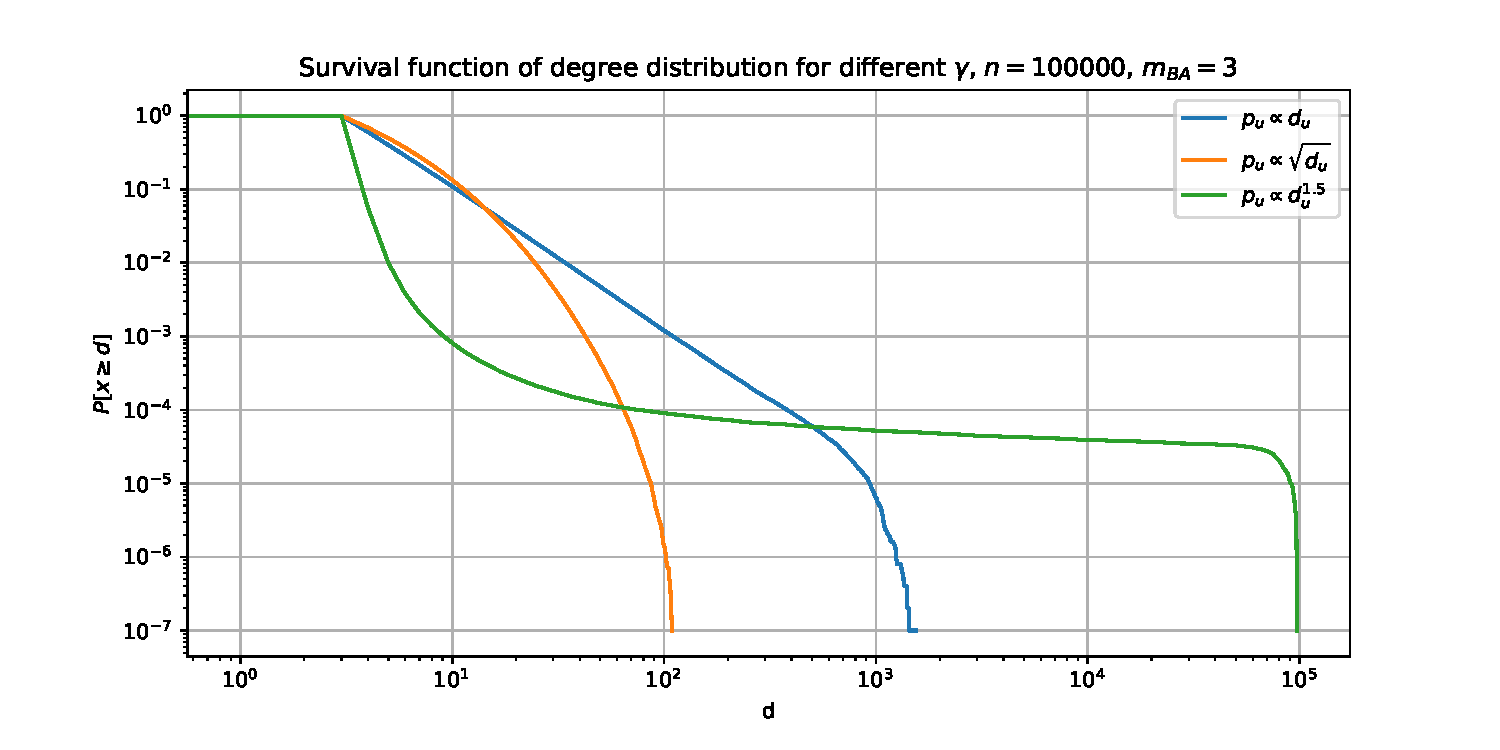
\includegraphics[width=.55\linewidth]{deg_gammacomp}
	\caption{Comparison of degree distributions for different values of gamma}
	\label{fig:deg4_gammacomp}
\end{figure}

\pagebreak
 
\begin{algorithm}
	\caption{Optimized algorithm to generate BA for the case $p_u \propto d_u$}
	\label{algo:ba_opt}
\begin{algorithmic}[1]
	\Function{generateBA}{$n, m_{BA}$}
		
		\State $graph \gets$ sparse matrix, size $n\times n$
		\State $urn \gets$ vector, size $2 n m_{BA}$
		\\
		\State $u \gets 1$
		\While {$u < m_{BA}+1$} \Comment{generate a complete graph of $m_{BA}+1$ nodes}
		\State $graph[u][0...u] \gets 1$
		
		\State $urn[len(urn) ... len(urn)+m_{BA}] \gets u$
		
		\State $u \gets u+1$
		\EndWhile
		\\
		\\
		\While {$u < n$} \Comment{add a new node at each iteration}
		\\
			\State $choices \gets $ pick $m$ \textbf{random} elements from $ urn $ (no repetitions)
			\\
			\State $graph[u][choices] \gets 1$ \Comment{connect node $u$ to all nodes in $choices$}
			\\
			\State $urn[len(urn) ... len(urn)+m_{BA}] \gets u$
			\State $urn[len(urn) ... len(urn)+m_{BA}] \gets choices$

		
		\State $u \gets u+1$
		\EndWhile
		\\	
		\State \Return $graph+transpose(graph)$
		\EndFunction
\end{algorithmic}
\end{algorithm}

\begin{algorithm}
	\caption{Generate BA, recomputing each time the distribution}
	\label{algo:ba}
	\begin{algorithmic}[1]
		\Function{generateBA}{$n, m_{BA}, f(x)=x^\gamma$}
		
		\State $graph \gets$ sparse matrix, size $n\times n$
		\State $d_u \gets$ vector, size $n$, full of $m$ \Comment{$d_u$ is the degree of each node, initially set to $m_{BA}$}
		\State $p_u \gets$ vector, size $n$, full of $f(m_{BA})$
		\\ \Comment{$p_u$ is the probability \underline{not normalized} to pick a node}
		\\
		\State $sum\_p_u \gets 0$  \Comment{$sum\_p_u$ is the $\sum_{u}{p_u}$}
		
		\\
		\State $u \gets 1$
		\While {$u < m_{BA}+1$} \Comment{generate a complete graph of $m_{BA}+1$ nodes}
		\State $graph[u][0...u] \gets 1$
		
		\State $u \gets u+1$
		\EndWhile
		\\
		\State $sum\_p_u \gets (m_{BA}+1)*f(m_{BA})$ 
		\\\Comment{update the sum: added $m_{BA}$ nodes with degree $m_{BA}$}
		\\
		\While {$u < n$} \Comment{add a new node at each iteration}
		\\
		\State $choices \gets random\_choice(size=m_{BA},p=p_u[0...u], sum\_p=sum\_p_u)$
		\\
		\State $graph[u][choices] \gets 1$ \Comment{connect node $u$ to all nodes in $choices$}
		\\
		\State $sum\_p_u-=p_u[choices]$	\Comment{update the $d_u$, $p_u$ and $sum\_p_u$ after the addition}
		\State $d_u[choices]+=1$
		\State $p_u[choices]=f(d_u[choices])$
		\State $sum\_p_u +=p_u[choices]$
		\\
		
		\State $u \gets u+1$
		\EndWhile
		\\	
		\State \Return $graph+transpose(graph)$
		\EndFunction
	\end{algorithmic}

\end{algorithm}

\begin{algorithm}
	\caption{Function $random\_choice$ to perform sampling from a discrete distribution}
	\label{algo:ba_r_c}
	\begin{algorithmic}[1]
		\Function{random\_choice}{$size,p, sum\_p$}
		\State $cdf \gets $ vector, size $length(p)$
		\State $choices \gets $ vector, size $size$
		
		\State  $cdf[0]=p[0]$
		\\
		\State $i \gets 0$
		\While{$i<size$} \Comment{loop on the number of choices to make}
		\State $r \gets random()*sum\_p_u$ \Comment{$random()$ returns a $Uniform[0,1]$}
		\\
		\If{$r<cdf[j]$}\Comment{if $r$ was in the part of $ cdf $ already computed}
		\\
		\State $new \gets $ binary search in $cdf[0...j+1]$, such that $cdf[new]\leq r < cdf[new+1]$
		\Else
		\While{$cdf[j]<r$} \Comment{continue to compute the $cdf$}
		\State $j+=1$
		\State $cdf[j]\gets cdf[j-1] + p[j]$
		\EndWhile
		\\
		\State $new \gets j$ \Comment{since the while stopped, $j$ is inside the block}
		\EndIf
		\\
		\If{$new$ is not already in $choices$}
		\State $choices[i] \gets new$
		\State $i+=1$
		\EndIf
		\EndWhile
		\\
		\State \Return $choices$
		\EndFunction
	\end{algorithmic}
	
\end{algorithm}


